\chapter{Analysis and Design}
\label{chap:analysis-and-design}

\bigskip

\begin{table}[tb] % placement: h for here, t for top, b for bottom
  \centering
  \begin{tabular}{l c}  % two columns: l for left, c for center, r for right
    Feature  & Benefit
    \\\hline
    Objects  & State encapsulation
    \\
    Generics & Code reuse
  \end{tabular}
  \caption{Advantages of Java}
  \label{tab:java-advantages}
\end{table}

\bigskip

\noindent
% LaTeX indents a new paragraph unless you specify \lstinline{\noindent}.
The Analysis part of this chapter will outline what features the robot will have and discuss the 
pros and cons of the technologies researched. 
The Design part will cover the choices made during the analysis and the reasoning why.

\bigskip


\begin{figure}[tb] % placement: h for here, t for top, b for bottom
  \centering
  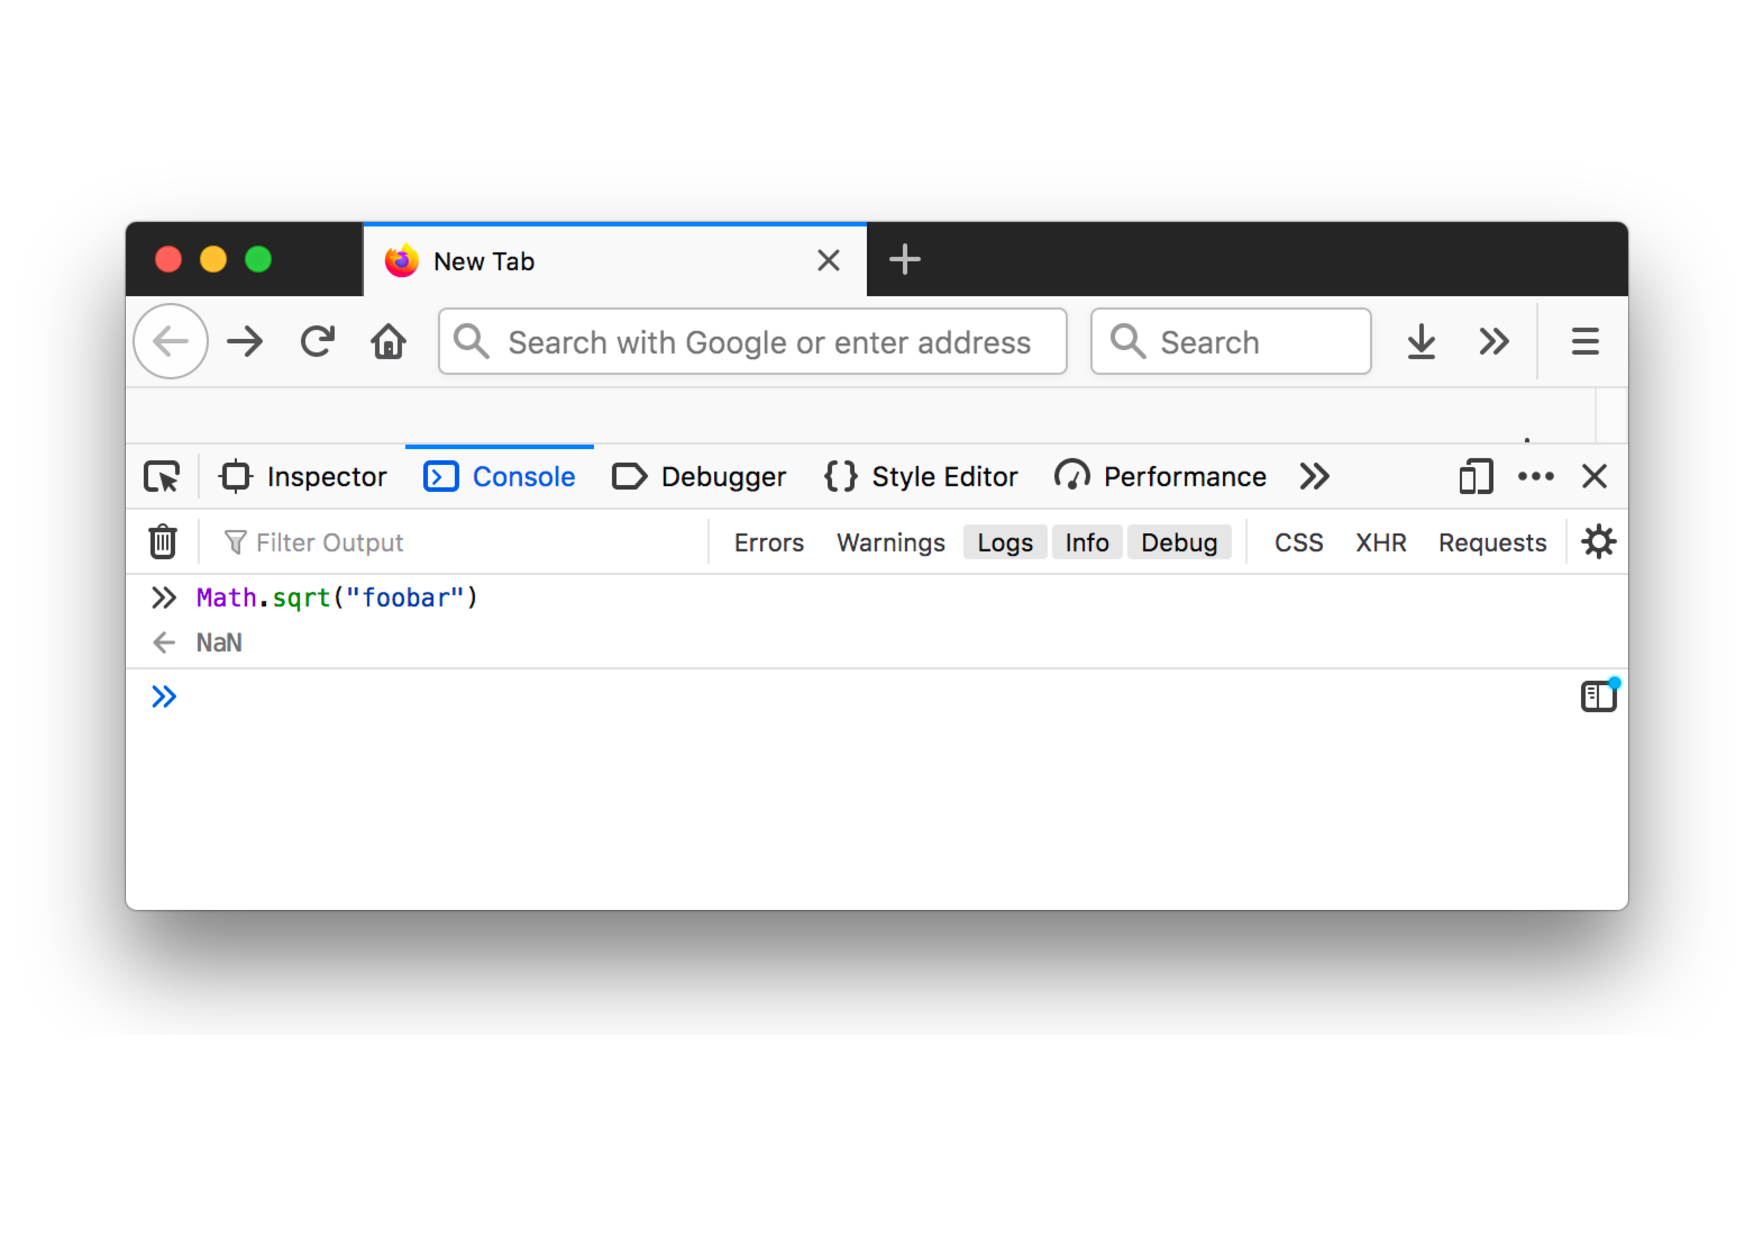
\includegraphics[width=.9\linewidth]{assets/firefox-js-console}
  \caption{The JavaScript console in Firefox }
  \label{fig:firefox-js-console}
\end{figure}
